\documentclass{beamer}
\usepackage[utf8]{inputenc}
\usetheme{Singapore}

%\title{Apresentação  ME}
%\subtitle{Delineamento e Otimização de Helicópteros de Papel }
%\author{Leonardo Uchoa, Hugo Calegari, Lara Acrani}
%\institute{Universidade Estadual de Campinas}
%\date{ }

%\titlegraphic{
\includegraphics[scale=0.2]{logo_unicamp}}

\begin{document}

\begin{frame}[plain]
    \title{Apresentação ME623}
    \subtitle{Delineamento e Otimização de Helicópteros de Papel}
    \institute{Universidade Estadual de Campinas}
    \date{ }
    \maketitle
    \small
    \begin{tabular}[t]{@{}l@{\hspace{3pt}}p{.32\textwidth}@{}}
        Autores: & Leonardo Uchoa \\
        &  Hugo Calegari \\
        &  Lara Acrani
    \end{tabular}%

    \begin{figure}
        
\includegraphics[scale=0.2]{logo_unicamp}
    \end{figure}
\end{frame}

\begin{frame}
    \frametitle{Sumário}
        \tableofcontents
\end{frame}

\section{Introdução}
    \begin{frame}
        \frametitle{Introdução}
        Pesquisa sobre otimização de tempo de queda para helicópteros feitos com papel no intuito de, futuramente, ter um modelo base relevante -ou seja, utilizando princípios bem fundamentados de sólida estrutura matemática- para replicação em massa.
    \end{frame}

\section{Objetivo}
    \begin{frame}
        \frametitle{Objetivo}
        O objetivo desta pesquisa é encontrar as especificações ótimas de maneira que, dentro um padrão, façam com que um Helicóptero de Papel, tenha o maior tempo de vôo possível em relação as demais características.
    \end{frame}

\section{Metodologia}
   \subsection{Técnica Estatística Empregada}
      \begin{frame}
           \frametitle{Metodologia}
               \framesubtitle{Técnica Estatística Empregada}
                 \begin{itemize}
                     \item As técnicas empregadas aqui seguem a metodologia estatística de Delineamento de Experimentos. Tal escolha é motivada pela sua capacidade de direcionar/apontar quais são os níves ótimos ao analisar cada combinação de fatores, o que é utilizado como "guia exploratório" desta pesquisa.

                     \item Em especial, o projeto será desenhado segundo um experimento fatorial, que nos permite avaliar cada possível combinação de fatores e seus respectivos níveis e extrair a melhor combinação entre fatores e níveis de todos os ensaios realizados.

                 \end{itemize}
      \end{frame}

    \subsection{Fatores}
        \begin{frame}
            \frametitle{Metodologia}
                \framesubtitle{Fatores}
                    Os fatores a serem analisados serão :

                        \begin{enumerate}
                            \item Formato da asa;
                            \item Comprimento da asa;
                            \item Largura da asa;
                            \item Material do helicóptero;
                            \item Peso do helicóptero;
                            \item Largura da banda.
                        \end{enumerate}

        \end{frame}

   \subsection{Níveis}
            \begin{frame}
                \framesubtitle{Níveis}
                    \frametitle{Metodologia}

                        Já os níveis, respectivos aos fatores, serão
                            \begin{itemize}
                                \item Com dobra e sem dobra;
                                \item 14 centímetros e 20 centímetros;
                                \item 4 centímetros e 6 centímetros;
                                \item Papel Sulfite e "Cartolina";
                                \item Clips tipo I e Clips tipo II;
                                \item 1 centímetro e 2 centímetros.
                            \end{itemize}
            \end{frame}

            \begin{frame}
                  \frametitle{Metodologia}
                     \framesubtitle{Experimento Fatorial e Aleatorização}
                        \begin{itemize}
                           \item Para tais níveis de fatores teremos, como proposto, um total de $\phi^k$ combinações entre características e tratamentos, onde $\phi$ é o número de níveis e k, a quantidade de fatores. Neste experimento, $k$ e $\phi$ assumem, respectivamente os valores 6 e 2.

                           \item Quanto à aleatorização, a ordem com que os helicóteros serão soltos será completamente aleatória, com o intuito de reduzir efeitos como, por exemplo, treinamento/condicionamento do operador que irá soltar o helicóptero.

                        \end{itemize}
            \end{frame}

            \begin{frame}
               \frametitle{Metodologia}
                  \framesubtitle{Aleatorização}
                     \begin{itemize}
                        \item A maneira para determinar a ordem de descida dos protótipos será realizando uma permutação randômica de todos os $2^6$ protótipos no software $R$.

                        \item Também ocorrerá aleatorização entre os operadores que irão soltar o helicóptero para, novamente, tentar amenizar o efeito de condicionamento do operador. Já esta escolha se dará ao utilizarmos um simulador de distribuição binomial, com 0.5 de probabilidade para cada operador.
                     \end{itemize}
            \end{frame}

\section{Modelos}
    \begin{frame}
        \frametitle{Metodologia}
            \framesubtitle{Modelos}
        \begin{figure}
            \label{fig:modelo tipo 1}
            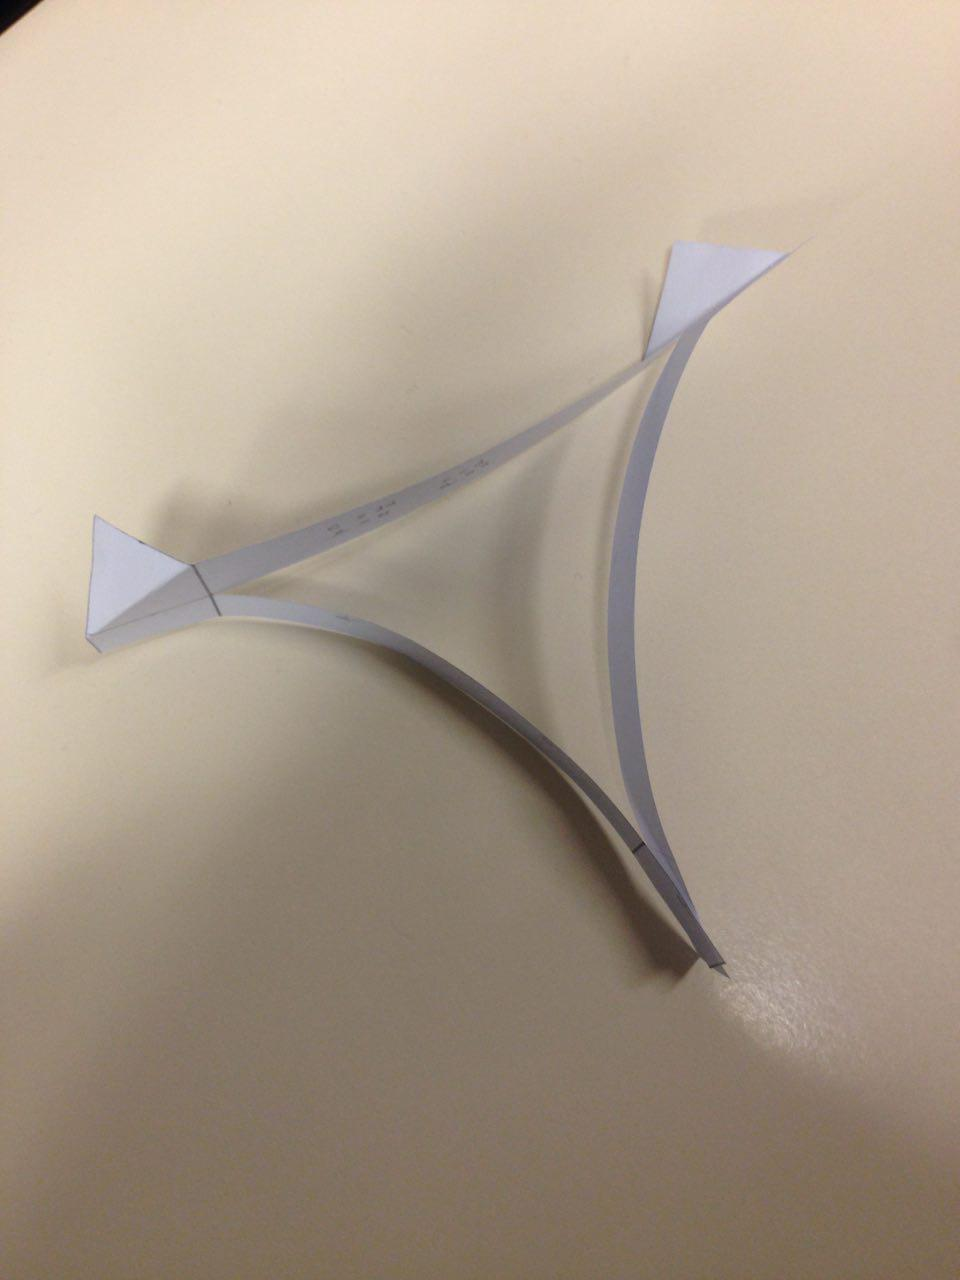
\includegraphics[scale=0.1]{foto01}
            \caption{Modelo tipo I}
        \end{figure}
    \end{frame}
    \begin{frame}
        \frametitle{Metodologia}
            \framesubtitle{Modelos}
        \begin{figure}
            \label{fig:modelo tipo 2}
            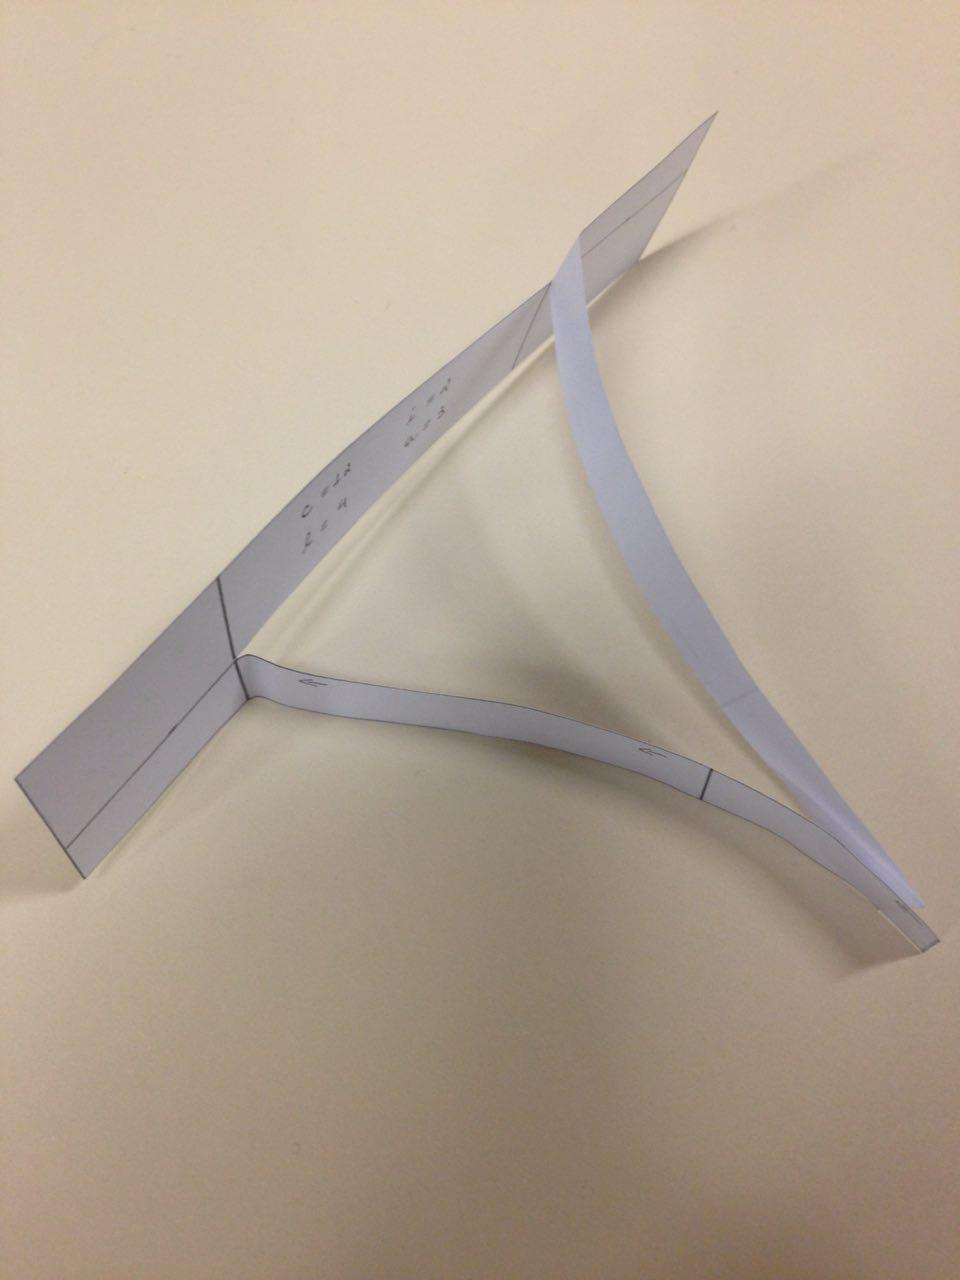
\includegraphics[scale=0.1]{foto02}
            \caption{Modelo tipo II}
        \end{figure}
    \end{frame}
    %\begin{frame}
        %\frametitle{Metodologia}
            %\framesubtitle{Modelos}
        %\begin{figure}
            %\label{fig:modelo tipo 3}
            %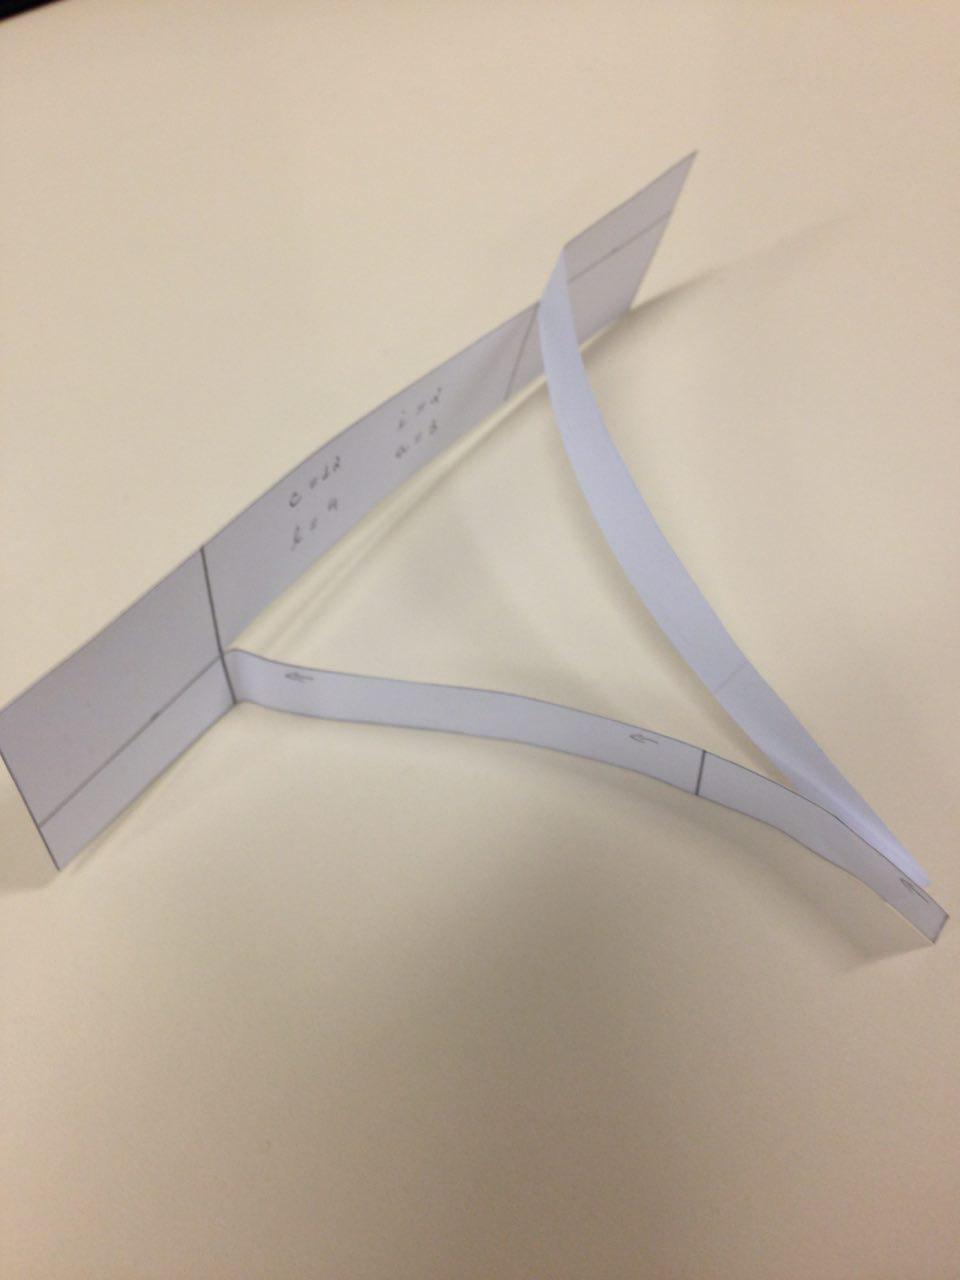
\includegraphics[scale=0.1]{foto03}
            %\caption{Modelo tipo III}
        %\end{figure}
    %\end{frame}

    \section{Resultados e Conclusões}
       \begin{frame}
         \frametitle{Resultados}
            Os resultados obtidos para cada ensaio, suas médias e variâncias e conclusão estão resumidos no arquivo .xsls que será aberto a seguir.
       \end{frame}

%\section{Conclusões}
%   \begin{frame}
%      \frametitle{Conclusões}




%   \end{frame}


\end{document}
